\paragraph*{Objectif du chapitre :}
\begin{itemize}
\item  Analyser les données brutes d'une série : caractère, type, modalité
\item  Déterminer et interpréter une fréquence, une moyenne, une médiane et  des quartiles.
\item  Trier des données brutes d'une série en dressant un tableau d'effectifs et en déterminant des classes
\end{itemize}

\section{Définitions et vocabulaire des statistiques}

La \textbf{population} est l'ensemble des individus sur lesquels portent l'étude statistique. \textsf{(Par exemple classe de seconde, hommes, habitants de la France \dots)}

\bigskip
Le \textbf{caractère} (ou \textbf{variable}) d'une série statistique est une propriété étudiée sur chaque individu :
\begin{itemize}
   \item  Lorsque le caractère ne prend que des valeurs (ou \textbf{modalités}) numériques, il est \textbf{quantitatif} :
   \begin{itemize}
       \item \textbf{discret} s'il ne peut prendre que des valeurs isolées \textsf{(notes, âge \dots )}
       \item \textbf{continu} dans le cas contraire \textsf{(poids, taille \dots )}. Dans ce cas on effectue souvent un regroupement des valeurs par \textbf{classes}.
    \end{itemize}
  \item  Sinon, on dit qu'il est \textbf{qualitatif} \textsf{(couleur des yeux, sport pratiqué \dots )}: les modalités ne sont pas des nombres.
\end{itemize}

\bigskip
\noindent A chaque valeur (ou classe) est associée un \textbf{effectif} $n$: c'est le nombre  d'individus associés à cette valeur.

\bigskip
Faire des \textbf{statistiques}, c'est recueillir, organiser, synthétiser, représenter et exploiter des données, numériques ou non, dans un but de comparaison, de prévision, de constat...

\bigskip
Les plus gros "consommateurs" de statistiques sont les \textbf{assureurs} (risques d'accidents, de maladie des assurés), les \textbf{médecins} (épidémiologie), les \textbf{démographes} (populations et leur dynamique), les \textbf{économistes} (emploi, conjoncture économique), les \textbf{météorologues} \dots

\bigskip

\begin{defi}{}{}
   On considère une série statistique à caractère quantitatif, dont les $p$ valeurs sont données par : \\
   $x_1$, $x_2$, \dots, $x_p$ d'effectifs associés $n_1$, $n_2$, \dots, $n_p$ avec $n_1+n_2+...+n_p=N$.
   \begin{itemize}
      \item  A chaque valeur (ou classe) est associée une \textbf{fréquence} $f_i$: c'est la proportion d'individus associés à cette valeur.
      \item  $f_i=\dfrac{n_i}{N}$ est un nombre compris entre $0$ et $1$, que l'on peut écrire sous forme de pourcentage.
      \item  L'ensemble des fréquences de toutes les valeurs du caractère s'appelle la \textbf{distribution des fréquences} de la série statistique.
   \end{itemize}
\end{defi}
\medskip

\begin{ex}{}{}
   Voici les notes obtenues à un contrôle dans une classe de $30$ élèves : (\textbf{Série A :}) \\ $2-3-3-4-5-6-6-7-7-7-8-8-8-8-8-9-9-9-9-9-9-10-10-11-11-11-13-13-15-16$ \\     
   On peut représenter cette série par un tableau d'effectifs, et le compléter par la distribution des fréquences : \\
   \renewcommand{\arraystretch}{1.5}   
   \begin{tabular}{|c|*{19}{C{0.4}|}}
      \hline       
      Notes & $1$ & $2$ & $3$ & $4$ & $5$ & $6$ & $7$ & $8$ & $9$ & $10$ & $11$ & $12$ & $13$ & $14$ & $15$ & $16$ & $17$ & $18$ & $19$ \\
      \hline
      Eff. & $0$ & $1$ & $2$ & $1$ & $1$ & $2$ & $3$ & $5$ & $6$ & $2$ & $3$ & $0$ & $2$ & $0$ & $1$ & $1$ & $0$ & $0$ & $0$ \\ 
      \hline
      Fréq. en \% & $0$ & $3$ & $7$ & $3$ & $3$ & $7$ & $10$ & $17$ & $20$ & $7$ & $10$ & $0$ & $7$ & $0$ & $3$ & $3$ & $0$ & $0$ & $0$ \\ 
      \hline
   \end{tabular}
\end{ex}
\medskip

\begin{rem}{}{}
   On peut vérifier que la somme des fréquences est égale à $1$ (ou à $100$ si on les exprime en pourcentages).
\end{rem}
\medskip

\noindent On peut aussi faire un regroupement par classe, ce qui rend l'étude moins précise, mais qui permet d'avoir une vision plus globale.
\medskip

\begin{ex}{}{}
   Toujours pour la \textbf{série A}, si on regroupe les données par classes d'amplitude $5$ points, on obtient :
   \begin{center}
   \renewcommand{\arraystretch}{1.5}
   \begin{tabular}{|*{6}{C{2}|}}
      \hline       
      Notes & $[~0~;~5~[$ & $[~5~;~10~[$ & $[~10~;~15~[$ & $[~15~;~20~[$ & total \\
      \hline
      Effectif & $4$ & $17$ & $7$ & $2$ & $30$ \\
      \hline
      Fréquence & $0,13$ & $0,57$ & $0,23$ & $0,07$ & $1$ \\
      \hline
   \end{tabular}
   \end{center}
\end{ex}

\section{Caractéristiques de position}

\subsection{Médiane (Vu en classe de $3^e$)}

\begin{defi}{}{}
   Soit une série statistique ordonnée dont les $n$ valeurs sont $x_1\leqslant x_2 \leqslant x_3 \leqslant \dots \leqslant x_n$.
   
   Une \textbf{médiane} est un nombre $Me$ qui permet de diviser cette série en deux sous-groupes de même effectif.
   \begin{itemize}
      \item  Si $n$ est \textbf{impair}, $M$ est la valeur de cette série qui est située au milieu, à savoir la valeur dont le rang est $\dfrac{n+1}{2}$, notée $x_{\frac{n+1}{2}}$.
      \item  Si $n$ est \textbf{pair}, $M$ est le centre de l'intervalle médian, qui est l'intervalle formé par les deux nombres situés \og au milieu \fg{} de la série, à savoir $x_{\frac{n}{2}}$ et $x_{\frac{n}{2}+1}$.
   \end{itemize}
\end{defi}
\medskip

\begin{ex}{}{}
   \begin{itemize}
      \item Une médiane de la série \og $2-5-6-8-9-9-10$ \fg{} est $8$.
      \item Une médiane de la série \og $2-5-6-8-9-9$ \fg{} est $7$.
      \item Une médiane de la série \og $2-5-6-6-9-10$ \fg{} est $6$.
   \end{itemize}
\end{ex}
\medskip

\subsection{Quartiles}

\begin{defi}{}{}
   Soit une série statistique, on appelle \textbf{quartiles} de la série un triplet de réels $(~Q_1~;~Q_2~;~Q_3~)$ qui sépare la série en quatre groupes de même effectif.
\end{defi}
\medskip

\begin{rem}{}{}
   Par définition, si $X$ est une série statistique, $Q_2 =Me(X)$.
\end{rem}
\medskip

\noindent La calculatrice donne les valeurs de $Q_1$, $Me$ et $Q_3$.

\noindent Nous verrons dans la partie \ref{Eff_Med} d'autres façons de trouver la médiane et les quartiles.

\begin{ex}{}{}
   Pour la \textbf{série A}, la calculatrice nous donne $Q_1=7$, $Me=8,5$ et $Q_3=10$.  
\end{ex}
\medskip

\subsection{Moyenne pondéré}

\begin{defi}{}{}
   Soit une série statistique à caractère quantitatif, dont les $p$ valeurs sont données par $x_1$, $x_2$, \dots, $x_p$ d'effectifs associés $n_1$, $n_2$, \dots, $n_p$ avec $n_1+n_2+...+n_p=N$.
   
   La \textbf{moyenne pondérée} de cette série est le nombre noté $\overline{x}$ qui vaut   $$\overline{x}=\dfrac{n_1x_1+n_2x_2+...+n_px_p}{n_1+n_2+...+n_p}=\dfrac{1}{N}\sum_{i=1}^{p}{n_ix_i}.$$
\end{defi}
\medskip

\begin{rem}{}{}
   Lorsque la série est regroupée en classes, on calcule la moyenne en prenant pour valeurs $x_i$ le \textbf{centre de chaque classe}; ce centre est obtenu en faisant la moyenne des deux extrémités de la classe.
\end{rem}
\medskip

\begin{ex}{}{}
   \begin{itemize}
     \item  Dans la \textbf{série A}, la moyenne du contrôle est égale à $$\overline{x} =\dfrac{2\times1+3\times2+\dots+16\times1}{30} =\dfrac{254}{30} \approx 8,47$$
     \item  si on regroupe par classe d'amplitude $5$ points, une estimation de la moyenne est : $$\overline{x} = \dfrac{2,5\times4+7.5\times17+\dots+17,5\times2}{30} =\dfrac{260}{30}\approx 8,67$$
   \end{itemize}
\end{ex}
\medskip

\begin{rem}{}{}
   On peut aussi calculer une moyenne à partir de la distribution de fréquences : $$\overline{x} =f_1x_1+f_2x_2+\dots +f_px_p =\sum_{i=1}^p f_ix_i.$$
\end{rem}
\medskip

\begin{prop}{}{}[Linéarité de la moyenne]

   \begin{itemize}
      \item  Si on ajoute (ou soustrait) un même nombre $k$ à toutes les valeurs d'une série, alors la moyenne de cette série se trouve augmentée (resp. diminuée) de $k$.
      \item  Si on multiplie (ou divise) par un même nombre non nul $k$ toutes les valeurs d'une série, alors la moyenne de cette série se trouve multipliée (resp. divisée) par $k$.
   \end{itemize}
\end{prop}

\begin{ex}{}{}
   On considère la \textbf{série A} :
   \begin{itemize}
      \item  Si on ajoute $1,5$ points à chaque note du contrôle, alors la moyenne de classe devient $$\overline{x}=8,47+1,5=9,97$$
      \item  Si on augmente chaque note de $10\%$, cela revient à multiplier chaque note par $1,1$, ce qui donne $$\overline{x}=8,47\times1,1=9,32$$
   \end{itemize}
\end{ex}

\begin{prop}{}{}[Moyenne par sous-groupes]

   Soit une série statistique, d'effectif total $N$, de moyenne $\overline{x}$. 
   
   Si on divise cette série en deux sous-groupes \textbf{disjoints} d'effectifs respectifs $p$ et $q$ (avec $p+q=N$) de moyennes respectives $\overline{x}_1$ et $\overline{x}_2$, alors on a : $$\overline{x}=\dfrac{p}{N} \times \overline{x}_1+\dfrac{q}{N} \times \overline{x}_2.$$
\end{prop}

\smallskip

\begin{ex}{}{}
   On suppose par exemple que les $12$ garçons de la classe de la \textbf{série A} ont obtenu une moyenne globale de $8$ sur $20$.
   \begin{itemize}
      \item  La moyenne du groupe formé par les filles de la classe vérifie : $9,47 =\dfrac{12}{30}\times 8+\dfrac{18}{30} \times \overline{m}_f$ .
      \item  Soit $\overline{m}_f=\dfrac{30}{18}\left(9,47-\dfrac{12}{30}\times 8\right)=10,45.$
   \end{itemize}
\end{ex}

\section{Caractéristiques de dispersion}

\begin{defi}{}{}
On appelle \textbf{étendue} d'une série discrète $X$ le réel défini par $e(X)=\max(X)-\min(X)$.
\end{defi}
\medskip

Il s'agit de la première mesure de la dispersion d'une série statistique. Son principal mérite a longtemps été d'exister, et de fournir une information sur la dispersion très simple à obtenir.

\begin{ex}{}{}
L'étendue de la \textbf{série A} est de $e(A)=16-2=14$.
\end{ex}
\medskip

\subsection{L'écart interquartile}

\begin{defi}{}{}
On appelle \textbf{intervalle inter-quartiles} l'intervalle $[~Q_1~;~Q_3~]$. 
   
\noindent L'amplitude de cet intervalle est appelée \textbf{écart inter-quartiles}. Cette valeur est l'indicateur de dispersion associé à la médiane.
\end{defi}
\medskip

\begin{ex}{}{}
   \begin{itemize}
      \item  Dans la \textbf{série A}, l'intervalle inter-quartile est l'intervalle $[~7~;~10~]$ dont l'écart vaut $10-7=3$.
      \item  Cet intervalle comprend donc la moitié des notes de la série située au centre de celle-ci.
   \end{itemize}
\end{ex}

\subsection{L'écart type}

\begin{defi}{}{}
\begin{itemize}
\item[-]L'écart type est un indicateur de dispersion associé à la moyenne : il mesure la dispersion des valeurs autour de la moyenne. Plus l'écart-type est grand, plus les valeurs sont dispersées et moins la moyenne représente de façon significative la série.
\item[-]L'écart type, noté $\sigma$, de la série statistique est obtenu à l'aide de la calculatrice.
\end{itemize}
\end{defi}

\medskip
Voir \textbf{Fiche méthode} : "Calcul de paramètres statistiques"

\begin{rem}{}{}
La connaissance des formules qui suivent sont facultatives

Il est possible de définir de manière rigoureuse l'écart type :
\begin{itemize}
\item[-]L'écart type $\sigma$ de la série statistique est défini comme la racine carrée de la variance $V$.
\[\sigma = \sqrt{V}\]
\item[-]La variance de la série statistique est :
\[V = \frac{n_{1}(x_{1}-\bar x)^{2}+...+n_{k}(x_{k}-\bar x)^{2}}{N}\]
La variance est aussi appelée la moyenne quadratique de la série centrée.
\end{itemize}
\end{rem}

\section{Effectifs et fréquences cumulés}

\begin{defi}{}{}
   Quand les valeurs d'un caractère quantitatif sont rangées dans l'ordre croissant, 
   \begin{itemize}
      \item  \textbf{L'effectif cumulé croissant [~respectivement décroissant~]} d'une valeur est la somme des effectifs des valeurs inférieures [~respectivement supérieures~] ou égales à cette valeur,
      \item  \textbf{la fréquence cumulée croissante [~respectivement décroissante~]} d'une valeur est la somme des fréquences des valeurs inférieures [~respectivement supérieures~] ou égales à cette valeur.
   \end{itemize}
\end{defi}
\medskip

\begin{ex}{}{}
On reprend l'exemple de la \textbf{série A} de notes du chapitre précédent, on obtient :
\smallskip

\noindent \renewcommand{\arraystretch}{1.6}
\begin{tabular}{|*{20}{c|}}
\hline
Notes & $01$ & $02$ & $03$ & $04$ & $05$ & $06$ & $07$ & $08$ & $09$ & $10$ & $11$ & $12$ & $13$ & $14$ & $15$ & $16$ & $17$ & $18$ & $19$ \\\hline
Eff. & $0$ & $1$ & $2$ & $1$ & $1$ & $2$ & $3$ & $5$ & $6$ & $2$ & $3$ & $0$ & $2$ & $0$ & $1$ & $1$ & $0$ & $0$ & $0$ \\\hline
E.C.C. & $0$ & $1$ & $3$ & $4$ & $5$ & $7$ & $10$ & \ovalbox{$15$} & \ovalbox{$21$} & $23$ & $26$ & $26$ & $28$ & $28$ & $29$ & $30$ & $30$ & $30$ & $30$ \\\hline
 E.C.D. & $30$ & $30$ & $29$ & $27$ & $26$ & $25$ & $23$ & $20$ & $15$ & $9$ & $7$ & $4$ & $4$ & $2$ & $2$ & $1$ & $0$ & $0$ & $0$ \\\hline
\end{tabular}
\smallskip
   
\noindent Ce tableau peut par exemple nous permettre de calculer une médiane de la série : 
\smallskip
  
\noindent l'effectif étant de $30$, on choisit la moyenne entre la $15^{ième}$ et la $16^{ième}$ note, lues dans la ligne des E.C.C.
\smallskip
   
\noindent On obtient $Me=\dfrac{8+9}{2}=8,5$.
\end{ex}
\medskip

\begin{ex}{}{}
Toujours pour l'exemple de la \textbf{série A} par classes, on s'intéresse cette fois-ci à la fréquence :

\begin{center}
\renewcommand{\arraystretch}{1.6}
\begin{tabular}{|c|*{4}{C{2}|}}\hline       
Notes & $[~0~;~5~[$ & $[~5~;~10~[$ & $[~10~;~15~[$ & $[~15~;~20~[$ \\\hline
Effectif & $4$ & $17$ & $7$ & $2$ \\\hline
Fréquence en \% & $13$ & $57$ & $23$ & $7$ \\\hline
F.c.c. & $13$ & $70$ & $93$ & $100$ \\\hline
F.c.d. & $100$ & $87$ & $3$ & $7$ \\\hline
\end{tabular}
\end{center}
\end{ex}

\pagebreak

\section{Représentation graphique d'une série statistique}

\subsection{Histogramme}

Lorsque le caractère étudié est \textbf{quantitatif} et lorsque les modalités sont regroupées en \textbf{classes}, on peut représenter la série par un \textbf{histogramme} : l'aire de chaque rectangle est alors proportionnelle à l'effectif (ou à la fréquence) associée à chaque classe.

Lorsque les classes ont la même \textbf{amplitude}, c'est la hauteur qui est proportionnelle à l'effectif.

\begin{ex}{}{}
   Histogramme de la \textbf{série A} pour laquelle les amplitudes sont toute égales à $5$ :
   \begin{center}
\definecolor{ffccww}{rgb}{1.,0.8,0.4}
\definecolor{qqwwtt}{rgb}{0.,0.4,0.2}
\definecolor{ccqqww}{rgb}{0.8,0.,0.4}
\definecolor{xdxdff}{rgb}{0.49019607843137253,0.49019607843137253,1.}
\definecolor{cqcqcq}{rgb}{0.7529411764705882,0.7529411764705882,0.7529411764705882}
\begin{tikzpicture}[line cap=round,line join=round,>=triangle 45,x=0.8cm,y=0.4cm]
\draw [color=cqcqcq,, xstep=0.8cm,ystep=0.8cm] (-0.5,-0.5) grid (20.5,18.);
\draw[->,color=black] (-0.5,0.) -- (20.5,0.);
\foreach \x in {1,2,3,4,5,6,7,8,9,10,11,12,13,14,15,16,17,18,19,20}
\draw[shift={(\x,0)},color=black] (0pt,2pt) -- (0pt,-2pt) node[below] {\footnotesize $\x$};
\draw[->,color=black] (0.,-0.5) -- (0.,18.);
\foreach \y in {2,4,6,8,10,12,14,16}
\draw[shift={(0,\y)},color=black] (2pt,0pt) -- (-2pt,0pt) node[left] {\footnotesize $\y$};
\draw[color=black] (0pt,-10pt) node[right] {\footnotesize $0$};
\clip(-0.5,-0.5) rectangle (20.5,18.);
\fill[color=xdxdff,fill=xdxdff,fill opacity=0.5] (16.,16.) -- (16.,14.) -- (17.,14.) -- (17.,16.) -- cycle;
\fill[color=ccqqww,fill=ccqqww,fill opacity=0.5] (0.,0.) -- (0.,4.) -- (5.,4.) -- (5.,0.) -- cycle;
\fill[color=qqwwtt,fill=qqwwtt,fill opacity=0.4] (5.,0.) -- (5.,17.) -- (10.,17.) -- (10.,0.) -- cycle;
\fill[color=ffccww,fill=ffccww,fill opacity=0.7] (10.,0.) -- (10.,9.) -- (15.,9.) -- (15.,0.) -- cycle;
\fill[color=xdxdff,fill=xdxdff,fill opacity=0.5] (15.,0.) -- (15.,2.) -- (20.,2.) -- (20.,0.) -- cycle;
\draw (16.,16.)-- (16.,14.);
\draw (16.,14.)-- (17.,14.);
\draw (17.,14.)-- (17.,16.);
\draw (17.,16.)-- (16.,16.);
\draw (0.,0.)-- (0.,4.);
\draw (0.,4.)-- (5.,4.);
\draw (5.,4.)-- (5.,0.);
\draw (5.,0.)-- (0.,0.);
\draw (5.,0.)-- (5.,17.);
\draw (5.,17.)-- (10.,17.);
\draw (10.,17.)-- (10.,0.);
\draw (10.,0.)-- (5.,0.);
\draw (10.,0.)-- (10.,9.);
\draw (10.,9.)-- (15.,9.);
\draw (15.,9.)-- (15.,0.);
\draw (15.,0.)-- (10.,0.);
\draw (15.,0.)-- (15.,2.);
\draw (15.,2.)-- (20.,2.);
\draw (20.,2.)-- (20.,0.);
\draw (20.,0.)-- (15.,0.);
\begin{scriptsize}
\draw[color=black] (16.5,13) node {\large{$\text{2 notes}$}};
\end{scriptsize}
\end{tikzpicture}
   \end{center}
\end{ex}

\begin{ex}{}{}
   Exemple d'un histogramme représentant la répartition des salaires dans une entreprise, l'amplitude des classes n'étant pas régulières :
   \begin{center}
\definecolor{ffzzqq}{rgb}{1.,0.6,0.}
\definecolor{ffttcc}{rgb}{1.,0.2,0.8}
\definecolor{xdxdff}{rgb}{0.49019607843137253,0.49019607843137253,1.}
\definecolor{ffwwqq}{rgb}{1.,0.4,0.}
\definecolor{qqzzcc}{rgb}{0.,0.6,0.8}
\definecolor{ffqqtt}{rgb}{1.,0.,0.2}
\definecolor{qqccqq}{rgb}{0.,0.8,0.}
\definecolor{cqcqcq}{rgb}{0.7529411764705882,0.7529411764705882,0.7529411764705882}
\begin{tikzpicture}[line cap=round,line join=round,>=triangle 45,x=0.01cm,y=10.0cm]
\draw [color=cqcqcq,, xstep=1.0cm,ystep=1.0cm] (850.,-0.05) grid (2450.,0.65);
\draw[->,color=black] (850.,0.) -- (2450.,0.);
\foreach \x in {900.,1000.,1100.,1200.,1300.,1400.,1500.,1600.,1700.,1800.,1900.,2000.,2100.,2200.,2300.,2400.}
\draw[shift={(\x,0)},color=black] (0pt,2pt) -- (0pt,-2pt) node[below] {\footnotesize $\x$};
\clip(850.,-0.05) rectangle (2450.,0.65);
\fill[color=qqccqq,fill=qqccqq,fill opacity=0.5] (900.,0.) -- (900.,0.2) -- (1200.,0.2) -- (1200.,0.) -- cycle;
\fill[color=ffqqtt,fill=ffqqtt,fill opacity=0.6] (1200.,0.2) -- (1200.,0.3) -- (1400.,0.3) -- (1400.,0.) -- (1200.,0.) -- cycle;
\fill[color=qqzzcc,fill=qqzzcc,fill opacity=0.6] (1400.,0.3) -- (1400.,0.6) -- (1600.,0.6) -- (1600.,0.) -- (1400.,0.) -- cycle;
\fill[color=ffwwqq,fill=ffwwqq,fill opacity=0.5] (1600.,0.4) -- (1800.,0.4) -- (1800.,0.) -- (1600.,0.) -- cycle;
\fill[color=xdxdff,fill=xdxdff,fill opacity=0.5] (1800.,0.2) -- (2000.,0.2) -- (2000.,0.) -- (1800.,0.) -- cycle;
\fill[color=ffttcc,fill=ffttcc,fill opacity=0.6] (2000.,0.1) -- (2400.,0.1) -- (2400.,0.) -- (2000.,0.) -- cycle;
\fill[color=ffzzqq,fill=ffzzqq,fill opacity=0.5] (2200.,0.6) -- (2200.,0.5) -- (2300.,0.5) -- (2300.,0.6) -- cycle;
\draw (900.,0.)-- (900.,0.2);
\draw (900.,0.2)-- (1200.,0.2);
\draw (1200.,0.2)-- (1200.,0.);
\draw (1200.,0.)-- (900.,0.);
\draw (1200.,0.2)-- (1200.,0.3);
\draw (1200.,0.3)-- (1400.,0.3);
\draw (1400.,0.3)-- (1400.,0.);
\draw (1400.,0.)-- (1200.,0.);
\draw (1200.,0.)-- (1200.,0.2);
\draw (1400.,0.3)-- (1400.,0.6);
\draw (1400.,0.6)-- (1600.,0.6);
\draw (1600.,0.6)-- (1600.,0.);
\draw (1600.,0.)-- (1400.,0.);
\draw (1400.,0.)-- (1400.,0.3);
\draw (1600.,0.4)-- (1800.,0.4);
\draw (1800.,0.4)-- (1800.,0.);
\draw (1800.,0.)-- (1600.,0.);
\draw (1600.,0.)-- (1600.,0.4);
\draw (1800.,0.2)-- (2000.,0.2);
\draw (2000.,0.2)-- (2000.,0.);
\draw (2000.,0.)-- (1800.,0.);
\draw (1800.,0.)-- (1800.,0.2);
\draw (2000.,0.1)-- (2400.,0.1);
\draw (2400.,0.1)-- (2400.,0.);
\draw (2400.,0.)-- (2000.,0.);
\draw (2000.,0.)-- (2000.,0.1);
\draw (2200.,0.6)-- (2200.,0.5);
\draw (2200.,0.5)-- (2300.,0.5);
\draw (2300.,0.5)-- (2300.,0.6);
\draw (2300.,0.6)-- (2200.,0.6);
\begin{scriptsize}
\draw[color=black] (2250,0.45) node {\large{$\text{5 salariés}$}};
\end{scriptsize}
\end{tikzpicture}
\end{center}
	
On obtient le tableau suivant :
\begin{center}
\begin{tabular}{|*{7}{c|}}
\hline
Salaires & $[900;1200]$ &$[1200;1400]$& $[1400;1600]$ &$[1600;1800]$ & $[1800;2000]$ & $[2000;2400]$ \\\hline
Effectif & $30$ & $30$ & $60$ & $40$ & $20$ & $10$ \\\hline
\end{tabular}
\end{center}
\end{ex}

\newpage
\subsection{Nuage de points}

   Lorsque le caractère étudié est \textbf{quantitatif et discret}, on peut représenter la série par un \textbf{nuage de points} : chaque couple de valeurs est représenté par un point dans un repère orthogonal.

\begin{ex}{}{}
   Nuage de points de la \textbf{série A} : 
   
\definecolor{ffqqqq}{rgb}{1.,0.,0.}
\definecolor{cqcqcq}{rgb}{0.7529411764705882,0.7529411764705882,0.7529411764705882}
\begin{tikzpicture}[line cap=round,line join=round,>=triangle 45,x=0.9cm,y=1.0cm]
\draw [color=cqcqcq,, xstep=0.9cm,ystep=1.0cm] (-0.5,-0.5) grid (17.5,6.5);
\draw[->,color=black] (-0.5,0.) -- (18.,0.);
\foreach \x in {,1.,2.,3.,4.,5.,6.,7.,8.,9.,10.,11.,12.,13.,14.,15.,16.,17.}
\draw[shift={(\x,0)},color=black] (0pt,2pt) -- (0pt,-2pt) node[below] {\footnotesize $\x$};
\draw[->,color=black] (0.,-0.5) -- (0.,6.5);
\foreach \y in {,1.,2.,3.,4.,5.,6.}
\draw[shift={(0,\y)},color=black] (2pt,0pt) -- (-2pt,0pt) node[left] {\footnotesize $\y$};
\draw[color=black] (0pt,-10pt) node[right] {\footnotesize $0$};
\clip(-0.5,-0.5) rectangle (18.,6.5);
\begin{scriptsize}
\draw [color=ffqqqq] (2.,1.)-- ++(-3.0pt,-3.0pt) -- ++(6.0pt,6.0pt) ++(-6.0pt,0) -- ++(6.0pt,-6.0pt);
\draw [color=ffqqqq] (3.,2.)-- ++(-3.0pt,-3.0pt) -- ++(6.0pt,6.0pt) ++(-6.0pt,0) -- ++(6.0pt,-6.0pt);
\draw [color=ffqqqq] (4.,1.)-- ++(-3.0pt,-3.0pt) -- ++(6.0pt,6.0pt) ++(-6.0pt,0) -- ++(6.0pt,-6.0pt);
\draw [color=ffqqqq] (5.,1.)-- ++(-3.0pt,-3.0pt) -- ++(6.0pt,6.0pt) ++(-6.0pt,0) -- ++(6.0pt,-6.0pt);
\draw [color=ffqqqq] (6.,2.)-- ++(-3.0pt,-3.0pt) -- ++(6.0pt,6.0pt) ++(-6.0pt,0) -- ++(6.0pt,-6.0pt);
\draw [color=ffqqqq] (7.,3.)-- ++(-3.0pt,-3.0pt) -- ++(6.0pt,6.0pt) ++(-6.0pt,0) -- ++(6.0pt,-6.0pt);
\draw [color=ffqqqq] (8.,5.)-- ++(-3.0pt,-3.0pt) -- ++(6.0pt,6.0pt) ++(-6.0pt,0) -- ++(6.0pt,-6.0pt);
\draw [color=ffqqqq] (9.,6.)-- ++(-3.0pt,-3.0pt) -- ++(6.0pt,6.0pt) ++(-6.0pt,0) -- ++(6.0pt,-6.0pt);
\draw [color=ffqqqq] (10.,2.)-- ++(-3.0pt,-3.0pt) -- ++(6.0pt,6.0pt) ++(-6.0pt,0) -- ++(6.0pt,-6.0pt);
\draw [color=ffqqqq] (11.,3.)-- ++(-3.0pt,-3.0pt) -- ++(6.0pt,6.0pt) ++(-6.0pt,0) -- ++(6.0pt,-6.0pt);
\draw [color=ffqqqq] (13.,2.)-- ++(-3.0pt,-3.0pt) -- ++(6.0pt,6.0pt) ++(-6.0pt,0) -- ++(6.0pt,-6.0pt);
\draw [color=ffqqqq] (15.,1.)-- ++(-3.0pt,-3.0pt) -- ++(6.0pt,6.0pt) ++(-6.0pt,0) -- ++(6.0pt,-6.0pt);
\draw [color=ffqqqq] (16.,1.)-- ++(-3.0pt,-3.0pt) -- ++(6.0pt,6.0pt) ++(-6.0pt,0) -- ++(6.0pt,-6.0pt);
\end{scriptsize}
\end{tikzpicture}
\end{ex}

\subsection{Courbe des fréquences cumulées}

Enfin, Lorsque le caractère étudié est \textbf{quantitatif} et lorsque les modalités sont regroupées en \textbf{classes}, on peut effectuer la \textbf{courbe des fréquences cumulées} (croissantes ou décroissantes) appelée aussi \textbf{polygone} des fréquences cumulées.

\begin{ex}{}{}
   Polygone des fréquences cumulées croissantes et décroissantes de la \textbf{série A} :
   \begin{center} 
\definecolor{qqwuqq}{rgb}{0.,0.39215686274509803,0.}
\definecolor{qqqqff}{rgb}{0.,0.,1.}
\definecolor{ffqqqq}{rgb}{1.,0.,0.}
\definecolor{cqcqcq}{rgb}{0.7529411764705882,0.7529411764705882,0.7529411764705882}
\begin{tikzpicture}[line cap=round,line join=round,>=triangle 45,x=0.7cm,y=0.07cm]
\draw [color=cqcqcq,, xstep=0.7cm,ystep=0.7cm] (-0.5,-0.5) grid (20.5,105.);
\draw[->,color=black] (-0.5,0.) -- (20.5,0.);
\foreach \x in {,1,2,3,4,5,6,7,8,9,10,11,12,13,14,15,16,17,18,19,20}
\draw[shift={(\x,0)},color=black] (0pt,2pt) -- (0pt,-2pt) node[below] {\footnotesize $\x$};
\draw[->,color=black] (0.,-0.5) -- (0.,105.);
\foreach \y in {10,20,30,40,50,60,70,80,90,100}
\draw[shift={(0,\y)},color=black] (2pt,0pt) -- (-2pt,0pt) node[left] {\footnotesize $\y$};
\draw[color=black] (0pt,-10pt) node[right] {\footnotesize $0$};
\clip(-0.5,-11) rectangle (20.5,105.);
\draw [line width=1.2pt,color=ffqqqq] (0.,100.)-- (4.989099229436637,86.95740231355286);
\draw [line width=1.2pt,color=ffqqqq] (4.989099229436637,86.95740231355286)-- (10.,30.);
\draw [line width=1.2pt,color=ffqqqq] (10.,30.)-- (14.993325675717633,7.31464198297435);
\draw [line width=1.2pt,color=ffqqqq] (14.993325675717633,7.31464198297435)-- (20.,0.);
\draw [line width=1.2pt,color=qqqqff] (0.,0.)-- (5.011507493899451,12.587369255701622);
\draw [line width=1.2pt,color=qqqqff] (5.011507493899451,12.587369255701622)-- (10.,70.);
\draw [line width=1.2pt,color=qqqqff] (10.,70.)-- (15.011507493899451,92.40555107388344);
\draw [line width=1.2pt,color=qqqqff] (15.011507493899451,92.40555107388344)-- (20.,100.);
\draw [line width=1.2pt,dash pattern=on 4pt off 4pt,color=qqwuqq] (0.,50.)-- (8.251420655813899,49.87557561886803);
\draw [line width=1.2pt,dash pattern=on 4pt off 4pt,color=qqwuqq] (8.251420655813899,49.87557561886803)-- (8.266052948444905,0.);
\draw [dash pattern=on 4pt off 4pt] (5.011507493899451,12.587369255701622)-- (5.,0.);
\draw [dash pattern=on 4pt off 4pt] (10.,70.)-- (10.,0.);
\draw [dash pattern=on 4pt off 4pt] (15.011507493899455,92.40555107388346)-- (15.,0.);
\draw [dash pattern=on 4pt off 4pt] (5.011507493899451,12.587369255701622)-- (4.989099229436638,86.95740231355288);
\draw [line width=1.2pt,dash pattern=on 4pt off 4pt] (20.,100.)-- (20.,0.);
\begin{scriptsize}
\draw[color=qqwuqq] (8.2,-8) node {\large{$\text{Médiane}$}};
\draw[color=blue] (0.8,103) node {$\text{F.C.C.}$};
\draw[color=black] (1.5,102.8) node {$\text{et}$};
\draw[color=red] (2.2,103) node {$\text{F.C.D.}$};
\end{scriptsize}
\end{tikzpicture}

   \end{center}
   On peut grâce à ces polygones déterminer une médiane de la série de deux manières :
   \begin{itemize}
      \item  Soit en  déterminant le point du polygone d'ordonnée $50\%$ : on trouve environ $M =8,2$,
      \item  soit en lisant l'abscisse du point d'intersection des deux courbes.
   \end{itemize}
\end{ex}

\section{Médiane, quartile et représentations graphiques associées} \label{Eff_Med}

Dans la partie précédente, on a réussi a déterminer graphiquement une médiane d'une série statistique à caractère quantitatif continu.

En effet, il n'est pas possible pour ce type de série de la faire analytiquement. Cependant pour les série à caractère quantitatif discret, il est tout a fait possible de le faire "à la main".

\subsection{Calcul de médiane et de quartiles}

\begin{ex}{}{}
Les résultats d'une enquête sur le prix d'une baguette de pain dans 30 boulangeries d'une ville sont regroupés dans le tableau suivant.
\begin{center}
\renewcommand{\arraystretch}{1.9}
\begin{tabular}{|c|c|c|c|c|c|c|c|c|c|c|c|c|}
\hline 
Prix \textit{(en centimes d'euros)} & 70 & 75 & 80 & 85 & 90 & 95 & 100 & 105 & 110 & 115 & 120 & Total \\ 
\hline 
Nombres de boulangerie & 1 & 1 & 2 & 4 & 7 & 3 & 3 & 4 & 2 & 2 & 1 & 30 \\ 
\hline 
\end{tabular} 
\end{center}

\begin{methode}{}{}[Calcul de la médiane (avec $N$ pair)]\label{meth_med_pair}

L'effectif total de la série statistiques est de $30$ donc $N$ est pair.

\noindent Une fois les valeurs de la série statistique triées par ordre croissant, une médiane est donc la moyenne des deux valeurs du milieu.
\begin{itemize}
\item[-]La première valeur du milieu est la valeur située à la position $ \dfrac{30}{2} = \textcolor{S1}{15} $
\item[-]La deuxième valeur du milieu est la valeur située à la position $ \dfrac{30}{2}+1 = \textcolor{S1}{16} $
\end{itemize}

\noindent Pour pouvoir trouver facilement quelle valeur se situe en position $\textcolor{S1}{15}$ et $\textcolor{S1}{16}$, il faut dresser le tableau des Effectifs cumulés croissants (E.c.c.).
\begin{center}
\renewcommand{\arraystretch}{1.8}
\begin{tabular}{|c|c|c|c|c|c|c|c|c|c|c|c|c|}
\hline 
Prix \textit{(en centimes d'euros)} & 70 & 75 & 80 & 85 & \textcolor{S2}{90} & \textcolor{S2}{95} & 100 & 105 & 110 & 115 & 120 & Total \\ 
\hline 
Nombres de boulangerie & 1 & 1 & 2 & 4 & 7 & 3 & 3 & 4 & 2 & 2 & 1 & 30 \\ 
\hline 
E.c.c. & 1 & 2 & 4 & 8 & \textcolor{S1}{15} & \textcolor{S1}{18} & 21 & 25 & 27 & 29 & 30 & X \\ 
\hline 
\end{tabular} 
\end{center}

\noindent La $\textcolor{S1}{15^{e}}$ valeur de la série vaut donc $\textcolor{S2}{90}$ et la $\textcolor{S1}{16^{e}}$ valeur vaut $\textcolor{S2}{95}$.

\noindent On fait la moyenne de la $15^{e}$ valeur et la $16^{e}$ valeur pour obtenir la médiane:
\begin{eqnarray*}
Me &=& \frac{\textcolor{S2}{90}+\textcolor{S2}{95}}{2}\\ 
&=& \textcolor{S2}{92.5}
\end{eqnarray*}
\noindent La médiane de cette série statistique est de $\textcolor{S2}{92.5}$ centimes.

\noindent On peut en conclure que la moitié des baguettes de pain de la ville coute $92.5$ centimes ou moins.
\end{methode}

\begin{methode}{}{}[Calcul des quartiles]

L'effectif total de la série statistique est de $30$.
\begin{itemize}
\item[-]Le premier quartile est la première valeur située au delà de la position $ \dfrac{1}{4} \times 30 = 7.5 $ donc la $\textcolor{S1}{8^{e}}$ valeur.
\item[-]Le troisième quartile est la première valeur située au delà de la position $ \dfrac{3}{4} \times 30 = 22.5 $ donc la $\textcolor{S1}{23^{e}}$ valeur.
\end{itemize}
Pour pouvoir trouver facilement quelles valeurs se situent en position \textcolor{S1}{8} et \textcolor{S1}{23}, on reprend le tableau des Effectifs cumulés croissants (E.c.c.).
\end{methode}

\begin{center}
\renewcommand{\arraystretch}{1.8}
\begin{tabular}{|c|c|c|c|c|c|c|c|c|c|c|c|c|}
\hline 
Prix \textit{(en centimes d'euros)} & 70 & 75 & 80 & \textcolor{S2}{85} & 90 & 95 & 100 & \textcolor{S2}{105} & 110 & 115 & 120 & Total \\ 
\hline 
Nombres de boulangerie & 1 & 1 & 2 & 4 & 7 & 3 & 3 & 4 & 2 & 2 & 1 & 30 \\ 
\hline 
E.c.c. & 1 & 2 & 4 & \textcolor{S1}{8} & 15 & 18 & 21 & \textcolor{S1}{25} & 27 & 29 & 30 & X \\ 
\hline 
\end{tabular} 
\end{center}

\noindent Donc le premier quartile $Q_{1}$ vaut $\textcolor{S2}{85}$ et $Q_{3}$ vaut $\textcolor{S2}{105}$. 

\noindent On peut en conclure qu'au moins un quart des baguettes de pain ont un prix inférieur à $85$ centimes d'euros et au moins $75\%$ des baguettes ont un prix inférieur à un euros et cinq centimes
\medskip

\noindent On peut aussi calculer la valeur de l'écart interquartile :
\[Q_{3} - Q_{1} = 105 - 85 = 20\] 

\noindent On peut en conclure que la moitié des baguettes de pain sont dans une fourchette de prix de $20$ centimes d'euros

\end{ex}

\subsection{Représentation graphique associée à la médiane et aux quartiles}

Les valeurs extrêmes (minimum et maximum), la médiane et les deux quartiles permettent de partager une série en quatre parties contenant chacune environ un quart de l'effectif total. On a ainsi une idée de la répartition des valeurs de cette série.

\begin{methode}{}{}[Construction du diagramme en boite]
\begin{itemize}
\item  Tracer un axe qui \textbf{DOIT} être gradué en fonction de la série statistique étudiée.
\item  La « boite » est limitée par $Q_{1}$ et $Q_{3}$. Sa longueur est $Q_{3} - Q_{1}$
\item  Elle montre la médiane $Me$.
\item  Les « moustaches » sont limitées par les valeurs extrêmes.
\end{itemize}
\bigbreak

\begin{tikzpicture}
    \filldraw[fill=white] (2,0) rectangle (5,1);% draw the box
    \draw (3,1) -- (3,0) node[below]{$Me$};% draw the median
    \draw (5,0.5) -- (7,0.5);% draw right whisker
    \draw (2,0.5) -- (1,0.5);% draw left whisker
    \draw (7,0.39) -- (7,0.61);% draw vertical tab
    \draw (1,0.39) -- (1,0.61);% draw vertical tab
    \node[below] at (1,0.2) {$Min$};% label the hinge
    \node[below] at (7,0.2) {$Max$};% label the hinge
    \node[below] at (2,0) {$Q_{1}$};% label the hinge
    \node[below] at (5,0) {$Q_{3}$};% label the hinge
    %Commentaire
    \draw [thick,<->](2,-1) -- (5,-1);
    \node[below] at (3.5,-1.1) {Ecart interquartile};
    \draw [thick,<->](1,-2) -- (7,-2);
    \node[below] at (3.5,-2.1) {Etendue};
    % Axis
    \draw[thick,->] (-4,1.5) -- (12.1,1.5);
	\foreach \x in {-4,-3,-2,-1,0,1,2,3,4,5,6,7,8,9,10,11,12} 
		\draw(\x,1.6)--(\x,1.4) node [below]{$...$};  
\end{tikzpicture}
\end{methode}

\begin{ex}{}{}
En reprenant l'étude fait sur nos boulangeries ci-dessus, on a :
\begin{itemize}
\item[-]$Q_{1} = 85$ et $Q_{3} = 105$
\item[-]$Me = 92.5$
\item[-]$Min = 70$ et $Max = 120$
\end{itemize}

Le diagramme en boîte de cette série statistique est donc :
\bigbreak
\begin{center}
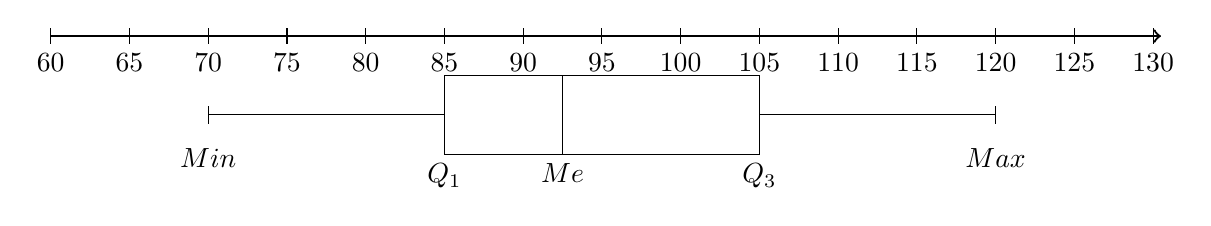
\begin{tikzpicture}
    \filldraw[fill=white] (1,0) rectangle (5,1);% draw the box
    \draw (2.5,1) -- (2.5,0) node[below]{$Me$};% draw the median
    \draw (5,0.5) -- (8,0.5);% draw right whisker
    \draw (1,0.5) -- (-2,0.5);% draw left whisker
    \draw (8,0.39) -- (8,0.61);% draw vertical tab
    \draw (-2,0.39) -- (-2,0.61);% draw vertical tab
    \node[below] at (-2,0.2) {$Min$};% label the hinge
    \node[below] at (8,0.2) {$Max$};% label the hinge
    \node[below] at (1,0) {$Q_{1}$};% label the hinge
    \node[below] at (5,0) {$Q_{3}$};% label the hinge
    % Axis
    \draw[thick,->] (-4,1.5) -- (10.1,1.5);
%	\foreach \x in {-4,-3,-2,-1,0,1,2,3,4,5,6,7,8,9,10,11,12} 
%		\draw(\x,-0.9)--(\x,-1.1) node [below]{..};  
	\draw(-4,1.6)--(-4,1.4) node [below]{60};
	\draw(-3,1.6)--(-3,1.4) node [below]{65};
	\draw(-2,1.6)--(-2,1.4) node [below]{70};
	\draw(-1,1.6)--(-1,1.4) node [below]{75};
	\draw(0,1.6)--(0,1.4) node [below]{80};
	\draw(1,1.6)--(1,1.4) node [below]{85};
	\draw(2,1.6)--(2,1.4) node [below]{90};
	\draw(3,1.6)--(3,1.4) node [below]{95};
	\draw(4,1.6)--(4,1.4) node [below]{100};
	\draw(5,1.6)--(5,1.4) node [below]{105};
	\draw(6,1.6)--(6,1.4) node [below]{110};
	\draw(7,1.6)--(7,1.4) node [below]{115};
	\draw(8,1.6)--(8,1.4) node [below]{120};
	\draw(9,1.6)--(9,1.4) node [below]{125};
	\draw(10,1.6)--(10,1.4) node [below]{130};
\end{tikzpicture}
\end{center}
\end{ex}

\begin{rem}{}{}
Il est souvent intéressant de tracer le diagramme en boîte de deux séries statistiques différentes sur le \textbf{même} axe gradué, afin de pouvoir mieux les comparer.
\end{rem}